%%%%%%%%%%%%%%%%%%%%%%%%%%%%%%%%%%%%%%%%%
% Arsclassica Article
% LaTeX Template
% Version 1.1 (1/8/17)
%
% This template has been downloaded from:
% http://www.LaTeXTemplates.com
%
% Original author:
% Lorenzo Pantieri (http://www.lorenzopantieri.net) with extensive modifications by:
% Vel (vel@latextemplates.com)
%
% License:
% CC BY-NC-SA 3.0 (http://creativecommons.org/licenses/by-nc-sa/3.0/)
%
%%%%%%%%%%%%%%%%%%%%%%%%%%%%%%%%%%%%%%%%%

%----------------------------------------------------------------------------------------
%	PACKAGES AND OTHER DOCUMENT CONFIGURATIONS
%----------------------------------------------------------------------------------------

\documentclass[
11pt, % Main document font size
letterpaper, % Paper type, use 'letterpaper' for US Letter paper
oneside, % One page layout (no page indentation)
%twoside, % Two page layout (page indentation for binding and different headers)
headinclude,footinclude, % Extra spacing for the header and footer
BCOR5mm, % Binding correction
]{scrartcl}

%%%%%%%%%%%%%%%%%%%%%%%%%%%%%%%%%%%%%%%%%
% Arsclassica Article
% Structure Specification File
%
% This file has been downloaded from:
% http://www.LaTeXTemplates.com
%
% Original author:
% Lorenzo Pantieri (http://www.lorenzopantieri.net) with extensive modifications by:
% Vel (vel@latextemplates.com)
%
% License:
% CC BY-NC-SA 3.0 (http://creativecommons.org/licenses/by-nc-sa/3.0/)
%
%%%%%%%%%%%%%%%%%%%%%%%%%%%%%%%%%%%%%%%%%

%----------------------------------------------------------------------------------------
%	REQUIRED PACKAGES
%----------------------------------------------------------------------------------------

\usepackage[
nochapters, % Turn off chapters since this is an article        
beramono, % Use the Bera Mono font for monospaced text (\texttt)
eulermath,% Use the Euler font for mathematics
pdfspacing, % Makes use of pdftex’ letter spacing capabilities via the microtype package
dottedtoc % Dotted lines leading to the page numbers in the table of contents
]{classicthesis} % The layout is based on the Classic Thesis style

\usepackage{arsclassica} % Modifies the Classic Thesis package

\usepackage[T1]{fontenc} % Use 8-bit encoding that has 256 glyphs

\usepackage[utf8]{inputenc} % Required for including letters with accents

\usepackage{graphicx} % Required for including images
\graphicspath{{Figures/}} % Set the default folder for images

\usepackage{enumitem} % Required for manipulating the whitespace between and within lists

\usepackage{lipsum} % Used for inserting dummy 'Lorem ipsum' text into the template

\usepackage{subfig} % Required for creating figures with multiple parts (subfigures)

\usepackage{amsmath,amssymb,amsthm} % For including math equations, theorems, symbols, etc

\usepackage{varioref} % More descriptive referencing

\usepackage[left=1in,right=1in,top=1in,bottom=1in]{geometry}

%\usepackage{titlesec}
%\titleformat{\section}{\normalfont\bfseries\spacedallcaps}{}{0pt}{}



%----------------------------------------------------------------------------------------
%	THEOREM STYLES
%---------------------------------------------------------------------------------------

\theoremstyle{definition} % Define theorem styles here based on the definition style (used for definitions and examples)
\newtheorem{definition}{Definition}

\theoremstyle{plain} % Define theorem styles here based on the plain style (used for theorems, lemmas, propositions)
\newtheorem{theorem}{Theorem}

\theoremstyle{remark} % Define theorem styles here based on the remark style (used for remarks and notes)

%----------------------------------------------------------------------------------------
%	HYPERLINKS
%---------------------------------------------------------------------------------------

\hypersetup{
%draft, % Uncomment to remove all links (useful for printing in black and white)
colorlinks=true, breaklinks=true, bookmarks=true,bookmarksnumbered,
urlcolor=webbrown, linkcolor=RoyalBlue, citecolor=webgreen, % Link colors
pdftitle={}, % PDF title
pdfauthor={\textcopyright}, % PDF Author
pdfsubject={}, % PDF Subject
pdfkeywords={}, % PDF Keywords
pdfcreator={pdfLaTeX}, % PDF Creator
pdfproducer={LaTeX with hyperref and ClassicThesis} % PDF producer
}

 % Include the structure.tex file which specified the document structure and layout

\hyphenation{Fortran hy-phen-ation} % Specify custom hyphenation points in words with dashes where you would like hyphenation to occur, or alternatively, don't put any dashes in a word to stop hyphenation altogether

%----------------------------------------------------------------------------------------
%	TITLE AND AUTHOR(S)
%----------------------------------------------------------------------------------------

\title{\normalfont{Mid-Term Report}} % The article title
\subtitle{\normalfont{$CS5350$ Machine Learning Exploratory Project}}

%\subtitle{Subtitle} % Uncomment to display a subtitle

\author{\spacedlowsmallcaps{Tyler Jones and Vijay Bajracharya}} % The article author(s) - author affiliations need to be specified in the AUTHOR AFFILIATIONS block

\date{} % An optional date to appear under the author(s)

%----------------------------------------------------------------------------------------

\begin{document}

%----------------------------------------------------------------------------------------
%	HEADERS
%----------------------------------------------------------------------------------------

\renewcommand{\sectionmark}[1]{\markright{\spacedlowsmallcaps{#1}}} % The header for all pages (oneside) or for even pages (twoside)
%\renewcommand{\subsectionmark}[1]{\markright{\thesubsection~#1}} % Uncomment when using the twoside option - this modifies the header on odd pages
\lehead{\mbox{\llap{\small\thepage\kern1em\color{halfgray} \vline}\color{halfgray}\hspace{0.5em}\rightmark\hfil}} % The header style

\pagestyle{scrheadings} % Enable the headers specified in this block

%----------------------------------------------------------------------------------------
%	TABLE OF CONTENTS & LISTS OF FIGURES AND TABLES
%----------------------------------------------------------------------------------------

\maketitle % Print the title/author/date block


\setcounter{tocdepth}{2} % Set the depth of the table of contents to show sections and subsections only

\tableofcontents % Print the table of contents

%----------------------------------------------------------------------------------------

 % Start the article content on the second page, remove this if you have a longer abstract that goes onto the second page

%----------------------------------------------------------------------------------------
%	Introduction
%----------------------------------------------------------------------------------------

\section{Introduction}

Traditional cybersecurity stacks consist of multiple layers of protection. Firewalls, endpoint protection, secure gateways, and authentication protocols are a few of the many tools used to protect a company’s network. Despite these efforts, the ever-evolving cybersecurity landscape continues to plague even the largest of companies in the world. To make monitoring and detection tasks easier, many businesses have started adopting intelligent and autonomous solutions into their security stacks. For our project, we want to perform a comparative analysis of various machine learning algorithms on public cybersecurity data. Moreoever, we want to assess their viability as an alternative approach to cyber-threat management. 


%------------------------------------------------

%----------------------------------------------------------------------------------------
%	Data Collection
%----------------------------------------------------------------------------------------

\section{Mid-Term Progress}
\subsection{Research}
 Heavily inspired by the paper on cybersecurity knowledge bases by Li et al (2020), our exploratory project is an appendage to a larger capstone project involving the autonomous detection and contextualization of network threats using knowledge graphs and neural networks. To support the results that we will generate using the neural network, we wanted to first form a baseline for comparison using traditional machine learning algorithms. Creating this baseline is the main goal for this project.\\
 In order to detect network intrusions, we had to familiarize ourselves with the most common types of network attacks. Since an entire network architecture has too many components to cover in one project, we decided to focus solely on network packet data for this exploratory project. For packet data, we searched for pre-existing public datasets that had specific attack types associated with network traffic. This is where we discovered the $UNSW\_NB15$ dataset, the details for which were published in five different papers that are listed in the references section of this report. Following the collection of data, we created a list of all the machine learning algorithms that we would be using for our project. So far, our list of algorithms contains decision tree, random forest, support vector machine, naive bayes, and k-nearest neighbors.

\subsection{Data Collection and Storage}
All of the algorithms that will be used in this project will utilize the $USNW\_NB15$ dataset. The dataset consists of raw network data packets that were generated in the Cyber Range Lab of the Australian Centre for Cyber Security based on real and synthesized attack patterns. It contains 100 gigabytes of network traffic but we will only be using a small subset of this data that was pre-sampled into testing and training data. We will be training our models on 82,332 labelled examples with 49 different features such as protocol, service, time to live, source to destination bytes etc. Moreover, the dataset is divided into 10 different attack families - normal, DoS, fuzzer, backdoor, exploit, renaissance, analysis, generic, shellcode and worms.\\\\ 
The training and testing sets are stored in the form of csv files. Due to the large size of these files, we had to compress the data using gzip. Every time an analysis is run, our program will decompress and extract the csv files into a local folder and use the relative paths to train the model and calculate classification errors.

\subsection{Data Preprocessing}
The packet data contains a mixture of both numerical and categorical data. Our first goal was to unify the dataset by mapping each categorical feature to a binary vector. To achieve this, we created a pandas dataframe from our csv files and split the data into feature vectors and ground truth labels. Then, we selected all feature vectors that were categorical in nature and used the sk-learn one-hot encoder to provide a numerical representation for categorical features. The converted features were then inserted back into the training set.

\subsection{Results}
So far, we have been able to use a decision tree classifier to train a model on our data and predict labels for the testing set. With a maximum tree depth set to 20, we were able to generate the following results: 

\begin{figure}[H]
    \centering
    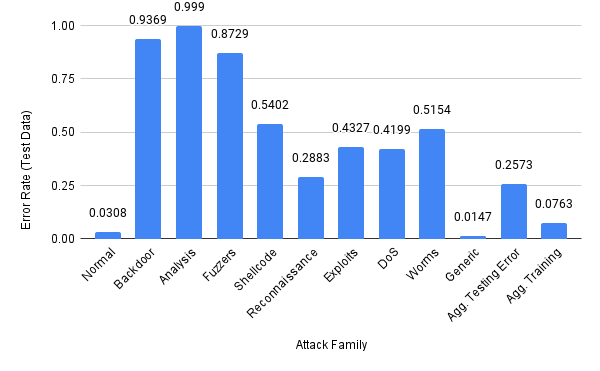
\includegraphics[scale=0.5]{decision_tree_chart.png}
    \caption{Comparison of classification error rates for each attack family}
    \label{fig:my_label}
\end{figure}

As we can see, while the aggregate testing error is 25\% and the training error is 0.07\%, the classifier performs very poorly on specific attack types. This might be a result of several factors including number of training examples, diversity of training examples, number of labels, the decision tree algorithm or the selected hyper-parameters.
%------------------------------------------------

%----------------------------------------------------------------------------------------
%	Future Plan
%----------------------------------------------------------------------------------------
\section{Plans for the Future}
The next step in our project is to add more algorithms specifically, random forest, support vector machine, naive bayes, and k-nearest neighbors. We also want to optimize existing algorithms such as decision trees by tuning hyper parameters like tree depth. Furthermore, we are considering using other ensemble techniques such as adaboost in addition to random forests. Once we have a suite of algorithms, we want to generate detailed reports for each one and compare the accuracy and running times of these algorithms. Moreover, to support our findings, we are also going to produce graphs and visualizations for all of the classification results.\\\\
From the results and visualizations, we can determine whether or not an intelligent solution for threat detection on a network is a viable approach for companies to adopt. These results will also act as a comparative baseline for the neural network that we will be building over the course of the senior capstone project.


%------------------------------------------------

%----------------------------------------------------------------------------------------
%	BIBLIOGRAPHY
%----------------------------------------------------------------------------------------
\section*{References}

1. Li, Kun, Huachun Zhou, Zhe Tu, and Bohao Feng. "CSKB: A Cyber Security Knowledge Base Based on Knowledge Graph." In International Conference on Security and Privacy in Digital Economy, pp. 100-113. Springer, Singapore, 2020.\\\\
2. Moustafa, Nour, and Jill Slay. "UNSW-NB15: a comprehensive data set for network intrusion detection systems (UNSW-NB15 network data set)." In 2015 military communications and information systems conference (MilCIS), pp. 1-6. IEEE, 2015.\\\\
3. Moustafa, Nour, and Jill Slay. "The evaluation of Network Anomaly Detection Systems: Statistical analysis of the UNSW-NB15 data set and the comparison with the KDD99 data set." Information Security Journal: A Global Perspective 25, no. 1-3 (2016): 18-31.\\\\
4. Moustafa, Nour, Jill Slay, and Gideon Creech. "Novel geometric area analysis technique for anomaly detection using trapezoidal area estimation on large-scale networks." IEEE Transactions on Big Data 5, no. 4 (2017): 481-494.\\\\
5. Moustafa, Nour, Gideon Creech, and Jill Slay. "Big data analytics for intrusion detection system: Statistical decision-making using finite dirichlet mixture models." In Data analytics and decision support for cybersecurity, pp. 127-156. Springer, Cham, 2017.\\\\
6. Sarhan, Mohanad, Siamak Layeghy, Nour Moustafa, and Marius Portmann. "Netflow datasets for machine learning-based network intrusion detection systems." arXiv preprint arXiv:2011.09144 (2020).

%----------------------------------------------------------------------------------------

\end{document}